\begin{mainquestion}{battery}{Power Transfer}
A typical CR2032 3 V coin-style battery (often used in watches or small electronic devices) has an internal source resistance $R_{s}$ of about $17~\si{\ohm}$ (seriously!) at room temperature. (While this value typically increases as the battery is depleted, we will consider it constant for this problem.)

\begin{center}
    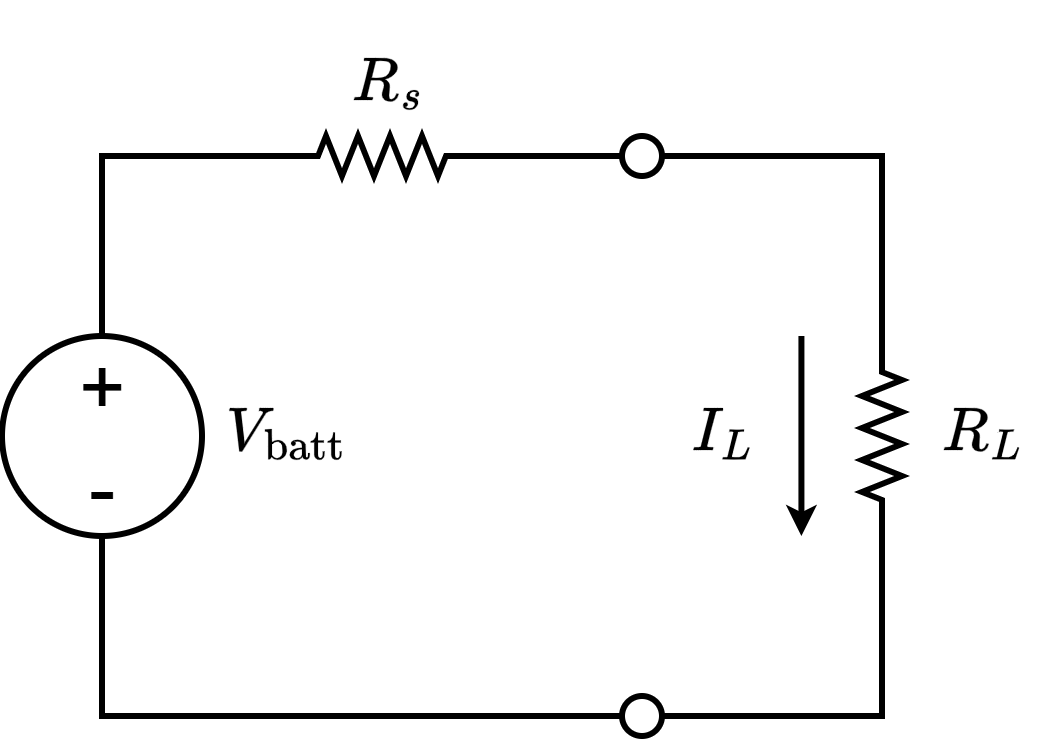
\includegraphics[width=4in]{circuit.png}
\end{center}

\begin{partquestion}{peakcurrent}{Using this battery, what is the peak current that could be driven through an external load $R_{L}$? What is $R_{L}$ in this scenario?}
\begin{answer}
The current is
\[
I=\frac{V_{\text{batt}}}{R_s+R_L},
\]
and to make this as large as possible, we make the denominator as small as possible. With $R_s$ fixed, we make
\[
R_L=0,
\]
so
\[
I=\frac{V_{\text{batt}}}{R_s} = \frac{3}{17}\,\si{\ampere}
    \approx 176\,\si{\milli\ampere}.
\]
\end{answer}
\end{partquestion}

\begin{partquestion}{peakpower}{Using this battery, what is the peak power that could be delivered through an external load $R_{L}$? What is $R_{L}$ in this scenario?}
\begin{answer}
Maximum power transfer occurs when
\[
R_L=R_s=17\,\si{\ohm},
\]
and the value of the power is
\[
P= \frac{V_L^2}{R_L} = \frac{(V_{\text{batt}}\frac{R_L}{R_s + R_L})^2}{R_L} = \frac{V_{\text{batt}}^2R_L}{(R_s + R_L)^2}
= \frac{V_{\text{batt}}^2}{4R_s}
=\frac{3^2}{4(17)}
=\frac{9}{68}\,\si{\watt}
\approx132\,\si{\milli\watt}.
\]
\end{answer}
\end{partquestion}

\begin{partquestion}{plotpower}{Plot the power delivered to $R_{L}$ as a function of $R_{L}$, from $0$ to $500~\si{\ohm}$.}
\begin{answer}
In the previous part, we derived the formula for the power dissipated in the load as:
\[P_{L} = \frac{V_{\text{batt}}^{2} R_{L}}{(R_{L} + R_{s})^{2}} = \frac{9 R_{L}}{(R_{L} + 17)^{2}}.\]

This can be plotted using MATLAB or some equivalent graphing program; the figure is shown below.

\begin{center}
    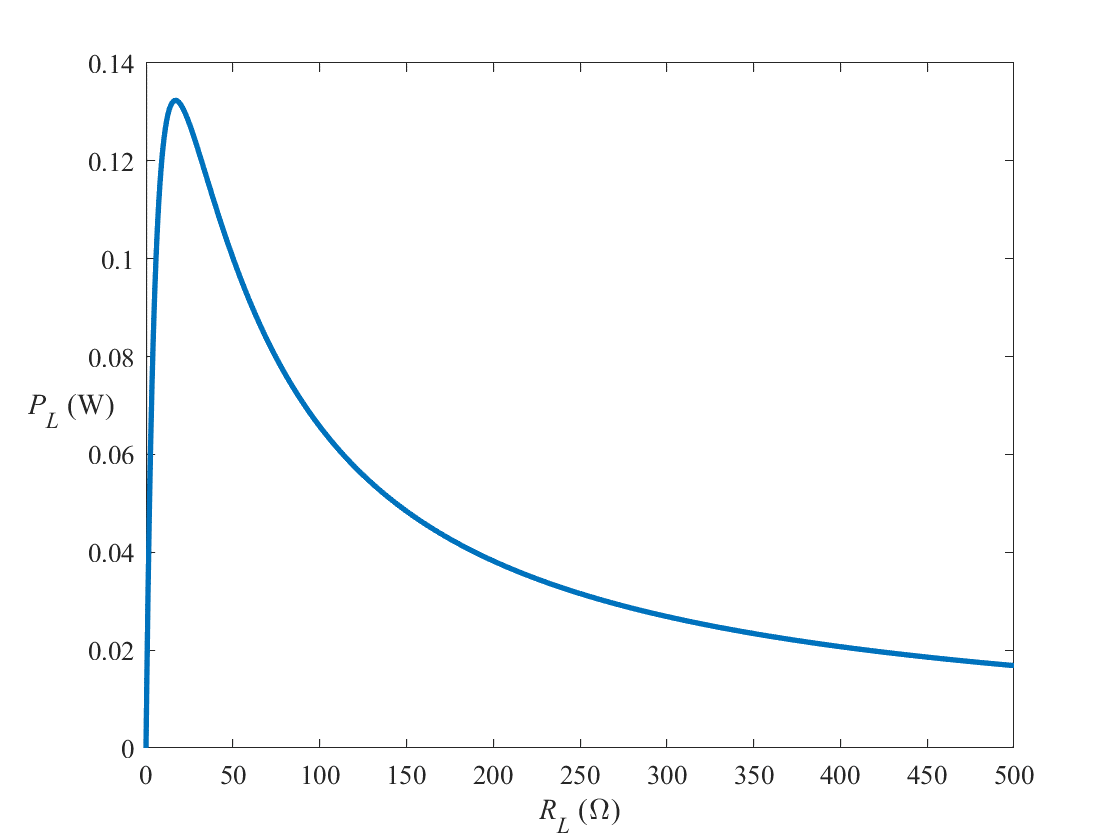
\includegraphics[width=5in]{plot.png}
\end{center}

Note the peak occurs at $17~\si{\ohm}$, as we expect. The power delivered to the load rolls off to zero as $R_L$ goes to zero.
\end{answer}
\end{partquestion}

\end{mainquestion}